\documentclass[letterpaper,12pt]{article}
\usepackage{array}
\usepackage{threeparttable}
\usepackage{geometry}
\usepackage{amsmath}
\geometry{letterpaper,tmargin=1in,bmargin=1in,lmargin=1.25in,rmargin=1.25in}
\usepackage{fancyhdr,lastpage}
\pagestyle{fancy}
\lhead{}
\chead{}
\rhead{}
\lfoot{}
\cfoot{}
\rfoot{\footnotesize\textsl{Page \thepage\ of \pageref{LastPage}}}
\renewcommand\headrulewidth{0pt}
\renewcommand\footrulewidth{0pt}
\usepackage[format=hang,font=normalsize,labelfont=bf]{caption}
\usepackage{listings}
\lstset{frame=single,
  language=Python,
  showstringspaces=false,
  columns=flexible,
  basicstyle={\small\ttfamily},
  numbers=none,
  breaklines=true,
  breakatwhitespace=true
  tabsize=3
}
\usepackage{amsmath}
\usepackage{amssymb}
\usepackage{amsthm}
\usepackage{harvard}
\usepackage{setspace}
\usepackage{float,color}
\usepackage[pdftex]{graphicx}
\usepackage{hyperref}
\hypersetup{colorlinks,linkcolor=red,urlcolor=blue}
\theoremstyle{definition}
\newtheorem{theorem}{Theorem}
\newtheorem{acknowledgement}[theorem]{Acknowledgement}
\newtheorem{algorithm}[theorem]{Algorithm}
\newtheorem{axiom}[theorem]{Axiom}
\newtheorem{case}[theorem]{Case}
\newtheorem{claim}[theorem]{Claim}
\newtheorem{conclusion}[theorem]{Conclusion}
\newtheorem{condition}[theorem]{Condition}
\newtheorem{conjecture}[theorem]{Conjecture}
\newtheorem{corollary}[theorem]{Corollary}
\newtheorem{criterion}[theorem]{Criterion}
\newtheorem{definition}[theorem]{Definition}
\newtheorem{derivation}{Derivation} % Number derivations on their own
\newtheorem{example}[theorem]{Example}
\newtheorem{exercise}[theorem]{Exercise}
\newtheorem{lemma}[theorem]{Lemma}
\newtheorem{notation}[theorem]{Notation}
\newtheorem{problem}[theorem]{Problem}
\newtheorem{proposition}{Proposition} % Number propositions on their own
\newtheorem{remark}[theorem]{Remark}
\newtheorem{solution}[theorem]{Solution}
\newtheorem{summary}[theorem]{Summary}
%\numberwithin{equation}{section}
\bibliographystyle{aer}
\newcommand\ve{\varepsilon}
\newcommand\boldline{\arrayrulewidth{1pt}\hline}
\setlength{\parindent}{4em}
\renewcommand{\baselinestretch}{2.0}
\setlength{\parskip}{0.5em}
\usepackage{indentfirst}


\begin{document}

\begin{titlepage}
    \begin{center}
        \vspace*{1cm}
        
        \Large
        \textbf{Do Covert Air Strikes Slow Terrorists Down?}
        
        \vspace{0.5cm}
        \Large
        The Effect of Covert Air Strike Fatalities on the Timing of Terrorist Attacks
        
        \vspace{0.5cm}
        
        \textbf{Soo Wan Kim}
        
        
        MACS 30200\\
        Final Paper
        
        \vspace{0.8cm}
        
        \Large
        Department of Social Sciences\\
        University of Chicago\\
        June 2017
        
    \end{center}
\end{titlepage}

\singlespacing

\begin{center}
    \Large
    \textbf{Abstract}
\end{center}
I investigate the relationship between fatalities from covert air strikes on terrorist groups and the subsequent timing of terrorist attacks, using Yemen in the years 2012 to 2015 as a case study. Specifically, I test the effect of fatalities from all covert air strikes in Yemen on the intervals in number of days between terrorist incidents. Using an original measure that estimates the cumulative long-term effects of covert strike fatalities, I estimate a simple linear model and a fixed effect model with years as fixed effects. I find that higher death counts in the past two, six, or twelve months are associated with shorter intervals between attacks - that is, higher fatalities appear to speed up terrorist attacks. The association is statistically significant at the 0.1 and 0.05 levels. Due to poor model fit and the small size of estimates, however, the findings are inconclusive.

\doublespacing

\section{Introduction}

In the years following the September 11 attacks, the US has carried out an unknown number of covert operations, mainly drone and other air strikes, to target terrorist groups in the Middle East, Africa, and the Afghanistan-Pakistan region. The US Department of Defense Dictionary defines a covert operation as an ``operation that is so planned and executed as to conceal the identity of or permit plausible denial by the sponsor.'' In other words, the White House releases information on the nature and extent of these operations only as it deems necessary, not as a matter of course.

Much debate and controversy surrounds the use of covert air strikes in the War on Terror. On the one hand, the use of guided missiles and unmanned aircrafts allows a high degree of precision and speed in killing enemy combatants, while greatly reducing the necessity of placing US personnel in dangerous positions. In theory, covert air strikes should reduce both military casualties and collateral damage to civilians, all the while neutralizing terrorist threats \cite{etzioni}. On the other hand, critics have pointed to their murky legality, substantial harm to civilians (in practice), and evidence of rising anti-US sentiment in regions targeted by covert strikes \cite{terrorfree,cavallaro,pew,khan}. 

The ethical and legal implications of covert strikes are beyond the scope of this paper. I address instead the strategic and tactical implications, specifically the ability of targeted killings using covert strikes to reduce the capabilities of militant organizations over time. There is a large volume of published literature on the use of targeted killings in counter-terrorism, but only a handful of large-n empirical studies focusing specifically on covert strikes. I review some of the major theoretical arguments and empirical findings from the literature below.

\subsection{Theory}

Scholars have cited four main theories for how targeted killings in counter-terrorism operations may affect militant organizations: deterrence, disruption, incapacitation, and backlash. The deterrence theory predicts that targeted killings will decrease terrorist activity for at least as long as crackdowns continue \cite{hafezhatfield,johnstonsarbahi}. Originating from the rational choice perspective, the deterrence theory makes the assumption that rational actors make decisions to maximize their net benefit \cite{lafree}. As the government cracks down on terrorist activity through killings, arrests, and other forms of repression, the costs of maintaining the insurgency increase, which then disincentivizes terrorists from further ``high-risk activism.'' Further, counter-terrorist operations deter the population from supporting terrorist groups by decreasing the groups' likelihood of success (Hafez and Hatfield 2006).

The disruption theory holds that targeted killings interfere with terrorist groups' normal operations and reduce their ability to plan and carry out attacks over time (Hafez and Hatfield 2006, Johnston and Sarbahi 2016). As groups are forced to allocate more time and resources to protecting and replacing important members, they become less able to mobilize resources for attacks. In addition, the loss of experienced and skilled members reduces the quality and success rate of attacks in both the long and short run.

Using a similar logic, the incapacitation theory predicts that targeted killings cripple terrorist groups by removing key individuals from the theater (LaFree et al. 2009, Hafez and Hatfield 2006). Leaders are assumed to play an important role in the groups' operational capabilities; thus, striking down leaders is expected to reduce the groups' effectiveness in the long run. In addition, targeted killings may deter individuals from joining terrorist movements, which will then reinforce the incapacitation effect (LaFree et al. 2009).

In contrast to the above three theories, the backlash theory predicts that targeted killings will increase future violence by magnifying grievances. Rather than deter terrorists, targeted killings may embolden them, triggering even more extreme violence. In addition, they may serve to increase pro-militant sympathies among local civilians, particularly where relations with the government have already soured. This will then allow militants to mobilize more resources and recruits (LaFree et al. 2009, Hafez and Hatfield 2006, Johnston and Sarbahi 2016).

Other scholars have focused on the organizational characteristics of militant groups and how the institutionalized processes or lack thereof within groups affect their resilience to targeted killings.	Price (2012) argues that targeting terrorist leaders is an effective counter-terrorism measure in that terrorist groups are ``violent, clandestine, and values-based organizations,'' which ``amplifie(s) the importance of leaders and make(s) leadership succession difficult'' (2012). He reasons that violent and clandestine groups are prone to forms of charismatic leadership, where leaders are less likely to delegate important tasks and lay out clear rules for succession, which then leads to fatal instability when leaders are killed. Jordan (2014) counters this argument, positing that targeting al-Qaeda's leadership is ineffective precisely because the group delegates tasks and follows rules. She cites bureaucratization and communal support as the key factors in the effectiveness of a leadership targeting strategy. She maintains that high levels of bureaucratization as typical of ``older and larger terrorist groups'' allows for smooth and stable transitions in leadership in the wake of a killing, while communal support contributes to group stability by facilitating recruitment and resource mobilization (2014). Likewise, Long (2014) finds that leadership targeting is effective against groups that are poorly institutionalized but much less effective against highly institutionalized groups.

\subsection{Empirical findings}

While targeted killings have been around for possibly as long as terrorism itself, the use of covert airstrikes in counter-terrorism is fairly new. The first known cases occurred in the early 2000s under the Bush administration, but arguably did not become a salient topic until the late 2000s and early 2010s when the Obama administration dramatically increased the use of precision air strikes in counter-terror operations abroad. In addition to the relative newness of the phenomenon, the difficulty of gathering accurate data on the incidence and location of strikes has meant that large-n studies on this topic are still few in number. As such, many questions are yet to be addressed.

Taken at face value, the studies that exist appear to contradict each others' findings. Lyall (2014), looking at the effects of US drone and other air strikes, found that recently struck areas in Afghanistan saw increased levels of insurgent attacks. Gill (2015), examining drone strikes only, found that increases in the incidence of drone strikes are associated with an increase in terrorist incidents in Pakistan. On the other hand, Johnston and Sarbahi (2016) found that drone strikes were effective in decreasing terrorist attacks in Pakistan. Jaeger and Siddique (2011) found that drone strikes had no significant effect on terrorist violence in Afghanistan, but significantly decreased terrorist violence in Pakistan.

Yet the differences may be explained partly by the differences in sampling. In particular, Jaeger and Siddique's findings suggest that the effects of targeted strikes on terrorist violence may be country or region-specific, as they found different results in Afghanistan and Pakistan. That said, it is striking that none of the studies address major theaters outside of the Afghanistan-Pakistan region, such as Yemen and Somalia. It is necessary to evaluate the effect of targeted strikes in multiple theaters in order to understand the potential roles of various geographical, political, and cultural factors, as well as more specific characteristics pertaining to the different groups and factions being targeted, on the effectiveness of targeted strikes. 

Moreover, the existing literature has yet to exhaust all the channels by which covert strikes negatively or positively impact terrorist organizations, and the specific effects that may be observed. The abovementioned studies mainly speak to the effect of the incidence of targeted killings on the incidence of terrorist activity. Some studies also deal with the spatial dimension, linking air strikes to terrorist incidents by region \cite{lyall,johnstonsarbahi}. However, no study has conducted a thorough examination of the effects of targeted strikes on the duration of the intervals between terrorist attacks. Gill (2015) and Johnston Sarbahi (2016) deal with duration models only as extensions to their main analyses and offer no conclusive results. Second, no study has directly examined the effect of covert strike fatalities as opposed to the incidence of strikes. In addition, there is a lack of attention to the long-term as opposed to the short-term effects of covert strikes.

\subsection{This study}

I attempt to draw inferences on the causal effects of covert strike fatalities on the intervals between terrorist attacks. I examine covert air strikes in Yemen ocurring between 2002 and 2015, and terrorist attacks between March 2012 and 2015. I limit the pool of terrorist attacks to those credibly linked to al-Qaeda in the Arabian Peninsula (AQAP), a Yemen-based branch of al-Qaeda that perpetrates a large proportion of all terrorist and insurgent violence in the Arabian Peninsula, and is also the primary target of counter-terror air strikes in Yemen. I limit the temporal scope for terrorist attacks to dates between March 2012 and end of 2015 as an attempt to control for exogenous change. The Yemeni Revolution, which is connected to the broader Arab Spring phenomenon, began roughly in January 27, 2011 and ended February 27, 2012. However, due to lack of data and detailed knowledge, I could not control for the political, social, economic, and other changes that took place in Yemen since 2012, including major military offensives by AQAP and counter-offensives by the Yemeni and Saudi regimes. Thus, my models, which only account for covert strike fatalities, offer only a tentative and highly limited explanation of the variation in intervals. 

Using a simple linear regression and year fixed effects models, I test the following hypotheses:
\begin{itemize}
  \item $H_0$: Fatalities from covert air strikes have no effect on the intervals between attacks.
  \item $H_1$: An increase in fatalities from covert air strikes shortens the intervals between attacks.
  \item $H_2$: An increase in fatalities from covert air strikes lengthens the intervals between attacks.
\end{itemize}

I find a significant negative association between covert strike fatalities and intervals between attacks, at the 0.1 and 0.05 level. In addition, I find evidence of heterogeneous variation in the tempo of attacks by year. However, the poor fit of the models and small magnitude of the estimated effects give pause to drawing any definite or generalizable conclusion.

\section{Data}

\subsection{AQAP attacks}

Data on AQAP attacks came from the Global Terrorism Database (GTD) managed at the University of Maryland. The GTD is one of the most detailed and comprehensive data sources for terrorist incidents around the world, and is freely accessible and extensively documented. The GTD defines terrorism as the ``\textit{the threatened or actual use of illegal force and violence by a non‐state actor to attain a political, economic, religious, or social goal through fear, coercion,
or intimidation}.'' Its criteria for inclusion in the database include, roughly speaking, intentionality on the part of the perpetrator, use or threat of violence, and sub-national actors as perpetrators. This broad definition of terrorism covers essentially all violent offensives by AQAP. While the GTD allows filtering based on more narrow criteria for what constitutes terrorism, it was not necessary for this study as I am interested in AQAP's offensive capabilities as a whole, not just their use of terrorist tactics.

Within the GTD I looked only at observations for incidents that took place in Yemen between March 1, 2012 and the end of 2015 for which the first perpetuating group is coded as ``Al-Qaida in the Arabian Peninsula'' or ``Al-Qaida in Yemen'' (a precursor to AQAP). In addition, I only used observations where the attribution of the attack to the group is not based on speculation or dubious sources ($guncertain1$ = 0). Based on these specifications, the number of individual terrorist attacks was 537. Because the unit of analysis for the timing of attacks is one day, attacks occurring on the same date were treated as one attack. This reduced the number of observations to 362.

Table 1 shows the number of attacks occurring each year, the average interval in days between each attack, and the minimum and maximum intervals. To note, the number of attacks measure counts every attack separately, but the interval measures treat attacks occuring on the same day as a single incident. Thus, the minimum interval is 1 day rather than 0 days.\\

\begin {table}[H]
\begin{center}
\caption {Summary of attacks by AQAP in Yemen, 2012 - 2015}
\begin{tabular}{rlrrl}
  \hline
Year & \# Attacks & Avg. interval & Interval range \\ 
&&(days)&(days)\\
  \hline
2012 & 104 & 4.1 & 1, 38 \\ 
  2013 &  87 & 5.2 & 1, 31 \\ 
  2014 & 235 & 2.6 & 1, 20 \\ 
  2015 & 111 & 4.7 & 1, 41 \\ 
  \hline
  All & 537 & 3.9 & 1, 41 \\ 
   \hline
\end{tabular}
\end{center}
\end {table}

Figures 1 and 2 show the distribution of intervals between attacks ocurring between 2009 to 2015 and 2012 to 2015, respectively. There is a notable decrease in the overall spacing between attacks starting in 2012, which could have been caused by political changes or even by the stepping up of counter-terror operations in the region. From 2012 on there is significantly less variation, though the overall pattern appears to vary from year to year. In particular, attacks are more numerous in 2014 and occur in quicker succession than in any other year, as the summary table corroborates.

\begin{figure}[htb!]
\begin{center}
\caption {Intervals between AQAP attacks in Yemen, 2009 - 2015}
  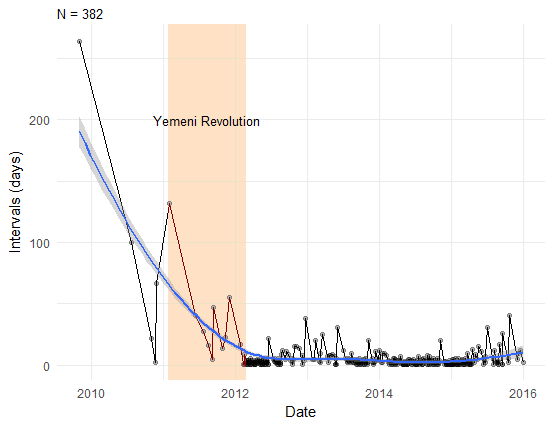
\includegraphics[width=3.5in]{intervals2009.png}
\end{center}
\end{figure}
\begin{figure}[htb!]
\begin{center}
\caption {Intervals between AQAP attacks in Yemen, Mar. 2012 - 2015}
  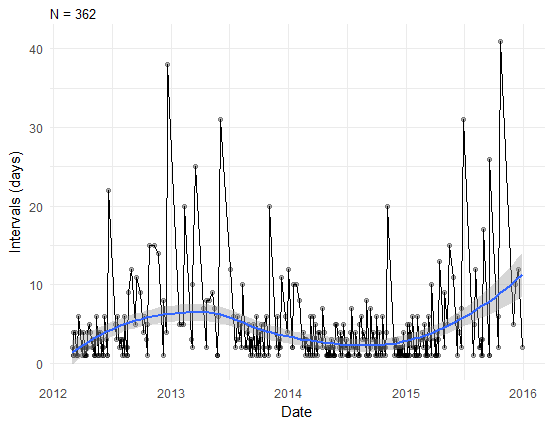
\includegraphics[width=3.5in]{intervals2012.png}
\end{center}
\end{figure}

Figure 3 shows the geographical spread of attacks, and figures 4 - 6 show the breakdown of attacks in terms of target type, weapon type, and suicidal intent per year. Attack targets coded as ``military'' include members of Yemeni or foreign state armed forces, police, and terrorists or non-state militia. Government targets include government workers and politicians, whether they are part of the ruling regime or a rival political party. All other target categories were coded as ``Other''. In terms of weapon type, the ``Unknown/Other'' category includes various weapon types such as biological, chemical, or radiological weapons, fake weapons, sabotage equipment, motor vehicles excluding car bombs, and unknown. An attack was coded as ``Yes'' for a suicide attack if there was evidence that the attacker did not intend to survive the attack. This does not necessarily imply a suicide bombing or any other deliberate self-martyrdom mission where the goal is to strictly die while killing the target.

Most attacks occur in the east and south. The composition of targets is similar across years, though there is an appreciable 17\% drop in the percentage of attacks aimed at military targets between 2014 and 2015, accompanied by a corresponding increase in government targets. Most attacks were carried out using explosives and firearms. The percentage of attacks using explosives appears to have decreased slightly over the years, as does the percentage of suicide attacks.

\newpage
\begin{figure}[htb!]
\begin{center}
\caption {Confirmed AQAP attacks in Yemen, Mar. 2012 - 2015}
  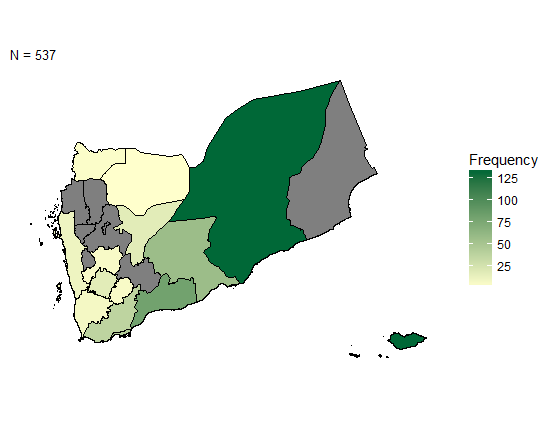
\includegraphics[width=3.5in]{attack_map.png}
\end{center}
\end{figure}

\begin{figure}[htb!]
\begin{center}
\caption {Percentage of attacks by target type}
  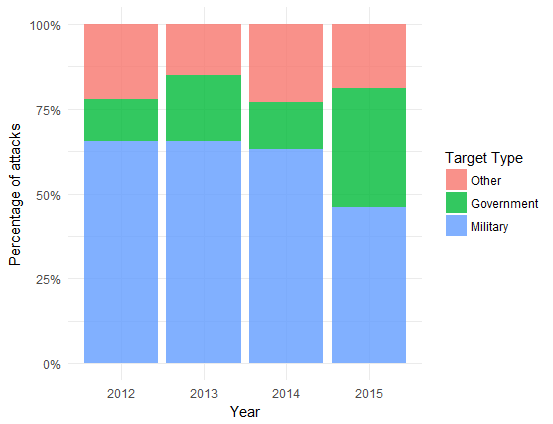
\includegraphics[width=3.5in]{attack_target.png}
\end{center}
\end{figure}

\begin{figure}[htb!]
\begin{center}
\caption {Percentage of attacks by weapon type}
  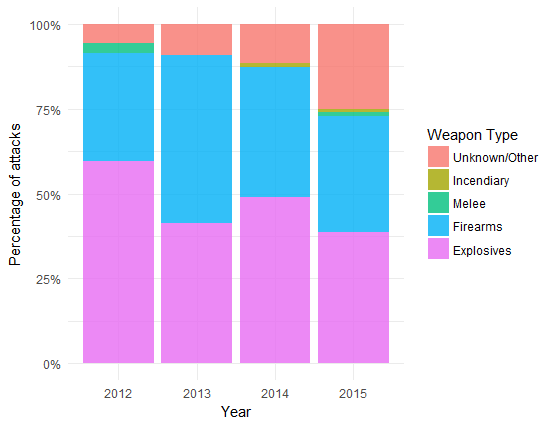
\includegraphics[width=3.5in]{attack_weapon.png}
\end{center}
\end{figure}

\begin{figure}[htb!]
\begin{center}
\caption {Use of suicide attacks over time}
  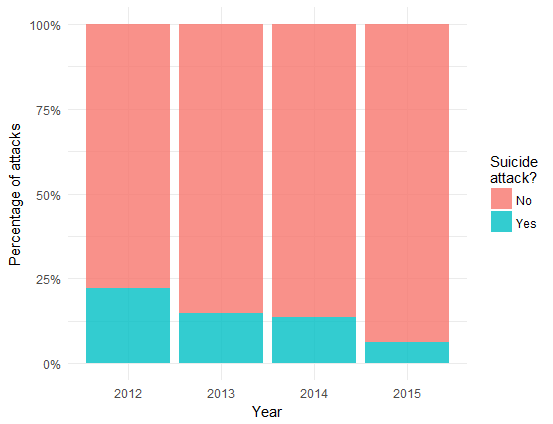
\includegraphics[width=3.5in]{attack_suicide.png}
\end{center}
\end{figure}

\newpage
\subsection{Covert strikes}

Covert strikes data came from the Bureau of Investigative Journalism (TBIJ), an independent watchdog organization that collects information on covert operations from media reports and other sources and compiles them into an online database. The database contains information on the locations of strikes and related fatalities. TBIJ recorded 210 covert strike incidents between 2002 and 2015, an incident being any event where a covert operation was carried out in a single date and location. One incident can include multiple strikes. The operations include ground operations as well as drone and air strikes, but the majority of observations pertain to drone and air strikes. 

In addition, I obtained the list of group leaders killed per incident from the New America Foundation's online Drone Wars database. I joined the number of group leaders killed per incident to each observation in the TBIJ data by date. Although the NAF and TBIJ databases contain similar information, I use the TBIJ data as the main source as it includes more incidents within the timeframe of interest.

Table 2 shows the number of incidents per year, as well as the percentage of incidents confirmed to be US operations (as opposed to covert operations carried out by regional powers, such as Yemen or Saudi Arabia), averages for minimum and maximum fatality estimates, and the number of group leaders killed. Group leaders include senior leaders and prominent ideologues, and any other high-profile member of AQAP. 

\begin{table}[ht!]
\centering
\caption {Summary of covert strike incidents in Yemen, 2002 - 2015}
\begin{tabular}{rlrrrrr}
  \hline
Year & \# Incidents & \% US Confirmed & Avg. killed & Avg. killed & \# Leaders killed \\ 
& & & (min.) & (max.) &\\
  \hline
2002 &   1 & 100 & 6 & 6 & 2 \\ 
2009 &   3 & 100 & 28.3 & 30.7 & 2 \\ 
2010 &   7 & 28.6 & 2.1 & 5.3 & 1 \\ 
2011 &  25 & 40 & 6.8 & 9.4 & 8\\ 
2012 &  78 & 43.6 & 6 & 8.5 & 23 \\ 
2013 &  32 & 68.8 & 3.6 & 5.5 & 10 \\ 
2014 &  32 & 56.2 & 4.6 & 6.7 & 0 \\ 
2015 &  32 & 65.6 & 3.4 & 4.9 & 3 \\ 
  \hline
All & 210 & 52.9 & 5.3 & 7.5 & 49 \\ 
   \hline
\end{tabular}
\end{table}

Figure 7 shows the distribution of fatalities from covert strikes. The measure used is the average of the minimum and maximum estimates for each incident. We see that the number of deaths is typically below 20, and further, that the number of civilian deaths is very small compared to the number of militant deaths. This reflects the high precision of the weaponry and tactics, and possibly limitations in reporting.

\begin{figure}[htb!]
\begin{center}
\caption {Reported casualties from covert strike incidents, 2009 - 2015}
  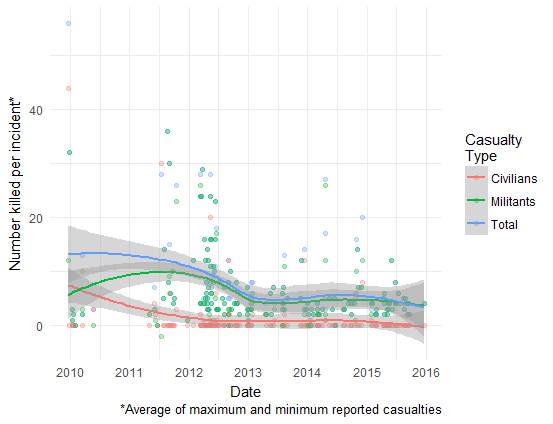
\includegraphics[width=3.5in]{strike_killed.png}
\end{center}
\end{figure}

Figure 8 shows that the covert strike operations are carried out primarily in the east and south, which is consistent with the geographical spread of terrorist attacks.

\begin{figure}[htb!]
\begin{center}
\caption {Location of covert strike incidents in Yemen, Mar. 2012 - 2015}
  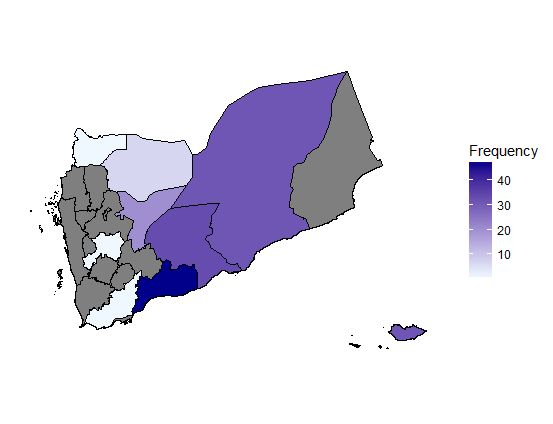
\includegraphics[width=3.5in]{strike_map.png}
\end{center}
\end{figure}

\newpage
\section{Methods}
I model the interval between one attack to another (in number of days) as a function of the cumulative effect of all covert strike fatalities incurred up to that point. To this end I employ a simple linear model and a fixed effects model. For both models I make the following simplifying assumptions:
\begin{itemize}
  \item \textbf{Assumption 1}: The effects of any given strike only lasts for a certain number of days; after this period has passed, the group recovers from any deaths caused by that strike.
  \item \textbf{Assumption 2}: Within the period where a strike is still relevant, its effects depreciate each passing month.
  \item \textbf{Assumption 3}: The death of a group leader has a greater effect than the death of a non-leader.
  \item \textbf{Assumption 4}: When multiple group leaders are killed in the same strike, the effect is multiplicative rather than additive.
  \item \textbf{Assumption 5}: The effect of the death of a non-leader is similar for militants and civilians.
\end{itemize}
Despite obvious differences in public perception regarding civilian deaths versus militant deaths, I argue that assumption 5 is not unreasonable in this context as the number of civilian deaths from covert air strikes in Yemen is very small, as shown in figure 7. In addition, the line between civilians and militants are often blurred, especially when militants and surrounding communities work together.

Also, while geographical factors likely play a role, I do not address them in this analysis. Lastly, I assume attacks always occur in ordered sequence; that is, the interval between attacks is always greater than 0. I treat attacks occuring on the same day as a single attack. 

For the simple linear regression I estimate the following:
\[log\left(interval_t\right) = \beta_0 + \beta_1log\left(killed_{ct}\right) \]
where for each time period $t$ in which an attack has occurred, $interval_{t}$ is the period of time in days until the next attack, and $killed_{ct}$ is the cumulative effect of all covert strike fatalities incurred up to and including period $t$.

This culumative effect is modeled as:
$$killed_{ct} = \sum_{n=t-x}^{t} (1 + \alpha)^{K_n}killed_{n}(1-\delta)^{D_{n}}$$
where $x$ is some fixed cutoff in difference in days, $\alpha$ is the added effect of the death of a group leader, $K_{n}$ is the number of group leaders killed in period $n$, $killed_{n}$ is the number of covert strike fatalities in period $n$, and $\delta$ is a depreciation constant by which the effect of an attack in a period depreciates in each subsequent period (due to new recruits, replacements, forgetting, etc.). $D_{n}$ is the 30-day difference between periods $n$ and $t$; I assume that the effects of an attack depreciate on a monthly basis. $D_{n}$ is calculated as follows:
$$D_{n} = floor((t - n)/30)$$
Thus, if $x$ = 30 the cumulative effect covers the deaths caused by covert strikes in the last thirty days and there is no depreciation effect. For $D_{n} > 1$ there is a depreciation effect and more recent deaths are weighed more heavily.

The parameters were set arbitrarily as follows: 
$$\alpha = 0.1; \delta = 0.6$$
and time difference $x$ was set at 60 (2 months), 180 (6 months), and 360 (1 year), respectively.

The fixed effects model employs the same model and specifications, but with added year fixed effects.

\section{Results}
\noindent\textit{Simple linear regression model}

The signs and significance of the estimates were similar across specifications $x$ = 60, 180, and 360. The results for $x$ = 60 and $x$ = 360 are included in Appendix A. I display the results for the model using $x$ = 180 in table 3 below:

\begin{table}[!htb]
\centering
\caption {LM of log intervals, $x$ = 180}
\begin{tabular}{rlrrrr}
  \hline
term & estimate & std.error & statistic & p.value \\ 
  \hline
(Intercept) & 1.54 & 0.13 & 11.64 & 0.00 \\ 
log(killed) & -0.07 & 0.04 & -1.74 & 0.08 \\ 
   \hline
\end{tabular}
\end{table}

The coefficient estimate indicates a very small negative association between the cumulative effect measure and the interval between attacks. A 1\% increase in the cumulative effect measure is associated with a 0.07\% decrease in the number of days until the next attack. Put differently, a 100\% increase in the cumulative effect measure is expected to decrease the interval by only 7\%. In fact, the range in predicted intervals across cumulative effects is quite narrow, as figure 9 shows. The association is significant at the 0.1 level. The R-squared value is low, at only 0.008876. \\

\begin{figure}[ht!]
\begin{center}
\caption {Predicted intervals without fixed effects, $x$ = 180}
  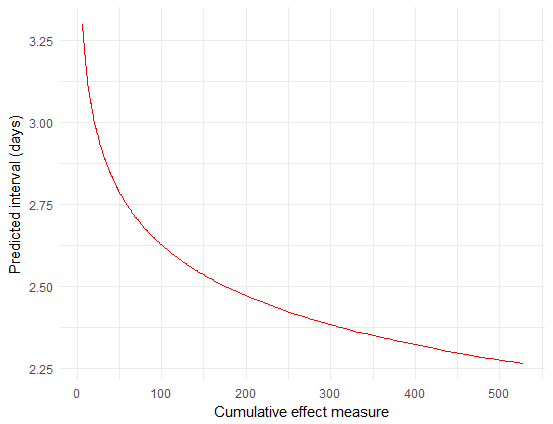
\includegraphics[width=3.5in]{pred_plot.png}
\end{center}
\end{figure}

\noindent\textit{Fixed effects model}

I estimate the same model as above with fixed year effects, using year 2012 as the baseline. Again, the signs and significance of coefficient estimates persisted across specifications  $x$ = 60, 180, and 360. Table 4 shows the output for the model setting $x$ = 180.

\begin{table}[htb!]
\centering
\caption {LM of log intervals with year fixed effects, $x$ = 180}
\begin{tabular}{rrrrr}
  \hline
&Estimate & Std. Error & t value & Pr($>$$|$t$|$) \\ 
  \hline
(Intercept) & 1.9097 & 0.2328 & 8.20 & 0.0000 \\ 
  log(killed) & -0.1274 & 0.0508 & -2.51 & 0.0126 \\ 
  factor(year)2013 & -0.0087 & 0.1285 & -0.07 & 0.9461 \\ 
  factor(year)2014 & -0.3569 & 0.1112 & -3.21 & 0.0015 \\ 
  factor(year)2015 & -0.1940 & 0.1248 & -1.55 & 0.1210 \\ 
   \hline
\end{tabular}
\end{table}

As with the simpler model, there is a small negative association between the cumulative effect measure and the attack interval. A 100\% increase in the cumulative effect measure is associated with a 12.7\% decrease in the number of days between attacks. The association is significant at the 0.05 level. In addition, relative to the base year 2012, years 2013 to 2015 are associated with slightly shorter intervals between attacks. The association is significant at the 0.01 level for year 2014. The R-squared is again low at 0.063.

\begin{figure}[htb!]
\begin{center}
\caption {LM of log attack intervals with year fixed effects}
  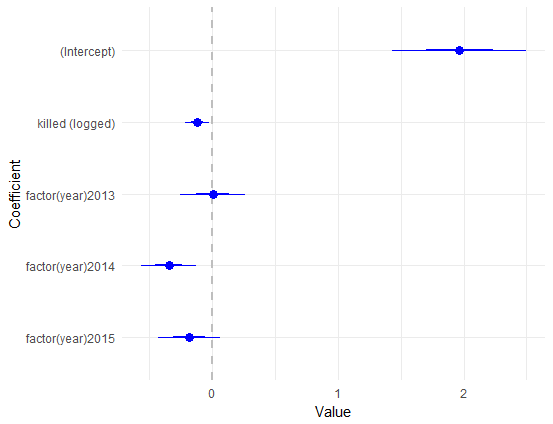
\includegraphics[width=3.5in]{coef_plot.png}
\end{center}
\end{figure}

As an extension to the main analysis, I tried estimating the models while limiting the pool of attacks to suicide bombings (setting $suicide$ = 1 and $weaptype1\_txt$ = ``Explosives/Bombs/Dynamite'') and attacks targeting the military, respectively. Limiting the pool of attacks by attack or target type did not lead to any substantive difference in the estimates, though they lost their statistical significance.  The regression outputs for these extension analyses are included in Appendix B.

\section{Discussion}

\noindent\textit{Interpretation of results}

The results indicate a small but significant negative association between my cumulative effect measure and the interval between attacks occuring on different days. In other words, higher covert strike fatalities and greater rates of leadership decapitation slightly decreases the amount of time between attacks. This appears to contradict the deterrence theory, which would predict a lower likelihood of carrying out attacks in any given period. However, it is consistent with the backlash theory, which predicts that militant groups will react with greater aggression in response to targeted killings, and consistent with Lyall (2014)'s findings. 

On the other hand, more attacks in shorter periods could also indicate increased vulnerability, which is more consistent with the disruption and incapacitation theories. For instance, weakened militant groups could opt for easier, less carefully planned attacks that require less time to prepare but have less impact. The trends across attacks support this theory to a limited extent; AQAP appears to be using explosives and suicide tactics less over time, as figures 5 and 6 show. Use of explosives and suicide attacks arguably requires more specific knowledge, greater training, and recruitment capabilities compared to other types of attacks, such as shootings or sabotage. However, the apparent change in tactics could also arise from other reasons not excluding random chance.

Regression results did not significantly differ when the period of relevance was changed from two months to six or twelve months. This is not surprising given that the depreciation rate was set at 60\%. More recent fatalities were weighed much more heavily than fatalities from older strikes.  

\noindent\textit{Limitations}

Due to the high frequency of attacks and the subsequent narrow distribution of intervals, measuring the intervals in days may be too blunt a measure to capture meaningful variation. A more fine-grained measure in hours or even minutes could provide more useful insight. 

Also, the distribution of attack intervals appear to differ from year to year. This in addition to the small R-squared values indicate that my models fail to account for important factors. A more refined model will take into account the volatile political situation in Yemen and other complex variations such as changes in military strategy and resource availability.

In addition to omitted variables bias, measurement bias is likely to play a role. The US government and other governments behind covert strikes offer little information about the extent and effects of covert operations. Media reports, on which the covert strike databases from the Bureau of Investigative Journalism and the New America Foundation are largely based, may not always provide full coverage or unbiased information. 

Lastly, I cannot rule out possible endogeneity between the independent and dependent variables. It is plausible that more frequent attacks would bring about more strikes and thus more fatalities, for instance.

\section{Conclusion}

My findings suggest that higher fatalities from covert strikes on militants speeds up rather than slows down terrorist attacks. However, the association between the cumulative effect measure and the intervals between attacks is slight at best. Also, the models explain only a tiny portion of the overall variation in attack intervals. As such, the findings from this study are inconclusive. A richer model containing control variables, and perhaps a more fine-grained measure of intervals between attacks, could allow for stronger inference. 

\nocite {gill,jaeger,johnston2012,jordan2014,long,price}

\bibliography{cov} 

\newpage
\appendix
\section{Regression output for $x$ = 60, 360}

\begin{table}[h!]
\centering
\caption {LM of log intervals, $x$ = 60}
\begin{tabular}{rlrrrr}
  \hline
 & term & estimate & std.error & statistic & p.value \\ 
  \hline
1 & (Intercept) & 1.51 & 0.12 & 12.85 & 0.00 \\ 
  2 & log(TotKilledMedW2 + 1) & -0.05 & 0.03 & -1.71 & 0.09 \\ 
   \hline
\end{tabular}
\end{table}

\begin{table}[h!]
\centering
\caption {LM of log intervals with year fixed effects, $x$ = 60}
\begin{tabular}{rlrrrr}
  \hline
 & term & estimate & std.error & statistic & p.value \\ 
  \hline
1 & (Intercept) & 1.70 & 0.19 & 9.07 & 0.00 \\ 
  2 & log(TotKilledMedW2 + 1) & -0.07 & 0.03 & -1.98 & 0.05 \\ 
  3 & factor(year)2013 & 0.07 & 0.12 & 0.55 & 0.59 \\ 
  4 & factor(year)2014 & -0.28 & 0.10 & -2.81 & 0.01 \\ 
  5 & factor(year)2015 & -0.12 & 0.12 & -1.05 & 0.29 \\ 
   \hline
\end{tabular}
\end{table}

\begin{table}[h!]
\centering
\caption {LM of log intervals, $x$ = 360}
\begin{tabular}{rlrrrr}
  \hline
 & term & estimate & std.error & statistic & p.value \\ 
  \hline
1 & (Intercept) & 1.58 & 0.16 & 9.84 & 0.00 \\ 
  2 & log(TotKilledMedW12 + 1) & -0.06 & 0.04 & -1.68 & 0.09 \\ 
   \hline
\end{tabular}
\end{table}

\begin{table}[h!]
\centering
\caption {LM of log intervals with year fixed effects, $x$ = 360}
\begin{tabular}{rlrrrr}
  \hline
 & term & estimate & std.error & statistic & p.value \\ 
  \hline
1 & (Intercept) & 1.96 & 0.27 & 7.37 & 0.00 \\ 
  2 & log(TotKilledMedW12 + 1) & -0.12 & 0.05 & -2.38 & 0.02 \\ 
  3 & factor(year)2013 & 0.01 & 0.13 & 0.04 & 0.96 \\ 
  4 & factor(year)2014 & -0.34 & 0.11 & -3.12 & 0.00 \\ 
  5 & factor(year)2015 & -0.18 & 0.12 & -1.46 & 0.15 \\ 
   \hline
\end{tabular}
\end{table}

\newpage
\section{Regression output for extension analyses}

\begin{table}[h!]
\centering
\caption {LM of log intervals, $x$ = 180 (suicide bombings)}
\begin{tabular}{rlrrrr}
  \hline
 & term & estimate & std.error & statistic & p.value \\ 
  \hline
1 & (Intercept) & 3.49 & 0.69 & 5.08 & 0.00 \\ 
  2 & log(TotKilledMedW6 + 1) & -0.19 & 0.15 & -1.25 & 0.22 \\ 
   \hline
&&&&&$n$ = 60
\end{tabular}
\end{table}

\begin{table}[h!]
\centering
\caption {LM of log intervals with year fixed effects, $x$ = 180 (suicide bombings)}
\begin{tabular}{rrrrr}
  \hline
 & Estimate & Std. Error & t value & Pr($>$$|$t$|$) \\ 
  \hline
(Intercept) & 2.7544 & 1.0215 & 2.70 & 0.0094 \\ 
  log(TotKilledMedW6 + 1) & -0.0800 & 0.1907 & -0.42 & 0.6766 \\ 
  factor(year)2013 & 0.9453 & 0.4751 & 1.99 & 0.0519 \\ 
  factor(year)2014 & 0.0470 & 0.4047 & 0.12 & 0.9081 \\ 
  factor(year)2015 & 0.7190 & 0.5709 & 1.26 & 0.2135 \\ 
   \hline
&&&&$n$ = 60
\end{tabular}
\end{table}

\begin{table}[h!]
\centering
\caption {LM of log intervals, $x$ = 180 (military targets)}
\begin{tabular}{rlrrrr}
  \hline
 & term & estimate & std.error & statistic & p.value \\ 
  \hline
1 & (Intercept) & 1.67 & 0.22 & 7.47 & 0.00 \\ 
  2 & log(TotKilledMedW6 + 1) & -0.05 & 0.05 & -0.91 & 0.36 \\ 
   \hline
&&&&&$n$ = 255
\end{tabular}
\end{table}

\begin{table}[h!]
\centering
\caption {LM of log intervals with year fixed effects, $x$ = 180 (military targets)}
\begin{tabular}{rrrrr}
  \hline
 & Estimate & Std. Error & t value & Pr($>$$|$t$|$) \\ 
  \hline
(Intercept) & 2.0597 & 0.3563 & 5.78 & 0.0000 \\ 
  log(TotKilledMedW6 + 1) & -0.0991 & 0.0652 & -1.52 & 0.1298 \\ 
  factor(year)2013 & 0.0536 & 0.1747 & 0.31 & 0.7593 \\ 
  factor(year)2014 & -0.4129 & 0.1481 & -2.79 & 0.0057 \\ 
  factor(year)2015 & -0.0272 & 0.1805 & -0.15 & 0.8801 \\ 
   \hline
&&&&$n$ = 255
\end{tabular}
\end{table}

\end{document}

